\section{Řešení}

Matice \bf{M} je velikosti \( \lr{T - p + 1} \times \lr{p + 1} \). Její předpis je
\[
    \bf{M} = 
    \begin{bmatrix}
        1 & y_{p - 1} & y_{p - 2} & \cdots & y_0 \\
        1 & y_p & y_{p - 1} & \cdots & y_1 \\
        \vdots & \vdots & \vdots & \ddots & \vdots \\
        1 & y_{T - 1} & y_{T - 2} & \cdots & y_{T - p}
    \end{bmatrix}
\]

Vektor hodnot \bf{b} je dán ze zadání. Jelikož musejí sedět rozměry při řešení soustavy, vektor \bf{b} má rozměr \( \lr{T - p + 1} \times 1 \). Jeho předpis vypadá následovně
\[
    \bf{b} =
    \begin{bmatrix}
        y_p \\
        y_{p + 1} \\
        \vdots \\
        y_T
    \end{bmatrix}
\]

Po vyřešení úlohy s použitím matic výše získáme následující řešení
\[ \min_a \lVert \bf{M} \bf{a} - \bf{b} \rVert^2 = 1.3621e^{-27}. \]

Pro řešení úlohy můžeme použít algoritmus využívající QR rozklad. Algoritmus má následující implementaci

\lstinputlisting{matlab/solve_ls.m}

kde funkce \verb|my_inversion| slouží jako náhrada za systémovou funkci \verb|inv| pro výpočet inverzní matice.

Pokud porovnáme řešení pomocí \( \bf{M} \setminus \bf{b} \) a výpočet pomocí QR rozkladu, získáme následující rozdíl:

\[ \lVert \hat{a_1} - \hat{a_2} \rVert = 6.3395e^{-13} \]

Výsledný graf porovnání syntetického a originálního zvuku gongu vypadá následovně

\begin{center}
    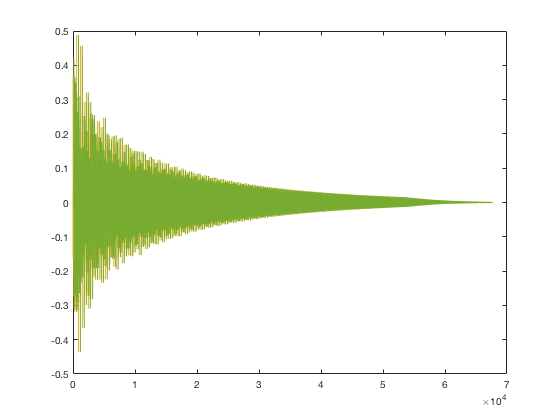
\includegraphics[width=0.73\textwidth]{graf.png}
\end{center}
